\chapter{Variables aleatorias}
  Hasta ahora nuestros sucesos han sido de varios tipos: $\{C,+\}$ en
  la moneda, nombres de periódicos, ángulos en una ruleta, número de
  veces que sale cara en el lanzamiento de una moneda etc\ldots.

  Necesitamos estandarizar de alguna manera todos estos sucesos. Una
  solución es asignar a cada suceso un cierto conjunto de
  números reales, es decir, convertir todos los sucesos en
  \emph{sucesos de números reales} para trabajar con ellos de forma
  unificada. Para conseguirlo utilizaremos  unas funciones que
  transformen los elementos del espacio muestral en números; esta funciones son las
  variables aleatorias.

  \section{Variables aleatorias}
 Comenzaremos dando una definición práctica de  variable aleatoria.

  \subsection{Definición de variable aleatoria}
  \begin{definition}
   De manera informal\footnote{Formalmente dado un espacio de probabilidad $(\Omega,\mathcal{F},P)$ y
    el espacio probabilizable\newline $(\RR,\mathcal{B}(\RR))$ una aplicación $X:\Omega\to\RR$ es una v.a. si y
    sólo si $X^{-1}(B)\in \mathcal{F}$ para todo $B\in\mathcal{B}(\RR)$.} una variable
    aleatoria (v.a.) es una aplicación que toma valores numéricos determinados por el resultado de un experimento aleatorio
   $$X:\Omega\to\RR$$
   \end{definition}

   \textbf{Notación}:
   \begin{itemize}
       \item Normalmente representaremos las v.a. por letras
       mayúsculas $X,Y,Z$\ldots
       \item Los valores que ``\emph{toman}'' las v.a. los
       representaremos por letras minúsculas (las mismas en principio)
       $x,y,z\ldots$
    \end{itemize}

\begin{example}
Lanzar un dado de seis caras entonces

$$\Omega=\{\epsdice{1}, \epsdice{2}, \epsdice{3}, \epsdice{4},  \epsdice{5},
\epsdice{6}\}$$
y  una v.a

$$X:\Omega\to\RR$$
 sobre este espacio queda definida por $X( \epsdice{1})=1,X( \epsdice{2})=2,X( \epsdice{3})=3,
 X( \epsdice{4})=4,X( \epsdice{5})=5,X( \epsdice{6})=6$. Ahora el suceso $A=\{ \epsdice{2},
  \epsdice{4}, \epsdice{6}\}$, es decir ``salir
número par'', es equivalente a $\{X=2,X=4,X=6\}$ y el suceso $B=\{ \epsdice{1},
  \epsdice{2}, \epsdice{3}\}$, es decir ''salir un número
inferior o igual a $3$" es  en términos de la v.a. $\{X=1,X=2,X=3\}$ o también $\{X\leq
3\}$.
\end{example}

\begin{example}
Consideremos el experimento lanzar una anilla al cuello de una botella. Si acertamos a
ensartar la anilla en la botella el resultado del experimento es \emph{éxito} y
\emph{fracaso} en caso contrario. El espacio muestral asociado a este experimento será
$\Omega=\{\mbox{éxito, fracaso}\}$. Construyamos la siguiente variable aleatoria:
$$X:\{\mbox{éxito, fracaso}\}\to\RR$$
definida por $X(\mbox{éxito})=1$ y  $X(\mbox{fracaso})=0$.
\end{example}

\subsection{Tipos de variables aleatorias}
       Hay dos tipos fundamentales de variables aleatorias, las discretas y las continuas.
       Damos a continuación una definición informal\footnote{
\begin{itemize}
\item La distinción entre variables aleatorias discretas y continuas es teóricamente más
sofisticada. En la práctica serán discretas aquellas variables a las que podamos asignar
probabilidades a los sucesos elementales y queden así descritas, siendo continuas las
``restantes''. En los problemas que trataremos en este curso esto será casi siempre así.
      \item  Hay variables aleatorias mixtas que, no por ser menos frecuentes, tienen menos
importancia.  Por ejemplo el tiempo que está ocupado un procesador atendiendo los trabajos
que llegan en una hora, si llega al menos un trabajo nos dará una v.a. continua pero si no
llega ningún trabajo el tiempo que está ocupado es cero en ese punto, que posiblemente
tenga probabilidad mayor que cero, la v.a. tiene un comportamiento discreto. Otro ejemplo
más artificial es el siguiente juego: lanzar un dado al aire y  si sale numero par anotar
el resultado mientras que  si sale impar lanzar un dardo a una diana y anotar la distancia
al centro. \end{itemize}} de estos tipos.
\begin{definition}
    \begin{enumerate}[a)]
    \item Una variable aleatoria es discreta si sólo puede tomar una cantidad numerable de valores con probabilidad
     positiva.
    \item La variables aleatorias continuas  toman  valores en intervalos.
\end{enumerate}
\end{definition}


  \begin{example}
      Son variables aleatorias discretas:
      \begin{itemize}
          \item  Número de artículos defectuosos en un cargamento.
          \item  Número de clientes que llegan a una ventanilla de un
          banco en una hora.
          \item  Número de errores detectados en las cuentas de una
          compañía.
          \item  Número de reclamaciones de una póliza de un seguro
          médico.
      \end{itemize}

       Son variables aleatorias continuas:
      \begin{itemize}
          \item  Renta anual de una familia.
          \item Cantidad de petróleo importado por un país
          \item  Variación del precio de las acciones de una compañía
          de telecomunicaciones.
          \item  Porcentaje de impurezas en un lote de productos
          químicos.
      \end{itemize}
\end{example}



\section{Distribuciones de probabilidad para v.a. discretas.}

Pasamos ahora a describir el comportamiento  de la v.a. Para ello utilizaremos distintas
funciones que nos darán algunas probabilidades de la variable aleatoria y que intentan
emular a las frecuencias relativas y relativas acumuladas que vimos para muestras. En el
caso discreto estas funciones son la de probabilidad, y  la de distribución.

\subsection{Función de probabilidad de una variable aleatoria
discreta}

En el caso discreto la función de probabilidad es la que nos da las probabilidades de los
sucesos elementales de la v.a.

\begin{definition}
La \emph{función de probabilidad}\footnote{También llamada función de cuantía o de masa
 de probabilidad,  inglés "\emph{ probability mass function}" por lo que se
 abrevia con el acrónimo \emph{pmf}, recordar esto cuando busquéis comandos en paquetes
estadísticos} de una variable aleatoria discreta $X$ a la que denotaremos por $P_{X}(x)$
está definida por\footnote{ Concretamente $P(X=x)=P(X^{-1}(x))$.}  $P_{X}(x)=P(X=x)$ es
decir la probabilidad de que $X$ tome el valor $x$. Si $X$ no asume ese valor entonces
$P_{X}(x)=0$. El conjunto $D_X=\{ x\in\RR \mid P_X(x)>0\}$ recibe el nombre de soporte o
dominio de la v.a. En el caso discreto lo más habitual es que $X(\Omega)=D_X$.
\end{definition}


\begin{example}
  En un dado de seis caras que se lanza una vez, en esta ocasión representaremos los
   sucesos elementales por el número de puntos de la cara obtenida,  tenemos que
  $\Omega=\{1,2,3,4,5,6\}$ y $X:\Omega\to \RR$ viene definida
  por  $X(i)=i$ para $i=1,2,3,4,5,6$. Supongamos que el dado está
  bien balanceado. Entonces
  $$P_{X}(1)=P_{X}(2)=P_{X}(3)=P_{X}(4)=P_{X}(5)=P_{X}(6)=\frac{1}{6}$$
  Concretamente:
  $$
  P_{X}(x)=
  \left\{
  \begin{array}{ll}
   \frac{1}{6} & \mbox{si } x=1,2,3,4,5,6\\
  0 & \mbox{en otro caso }
  \end{array}
  \right.
  $$
\end{example}

\begin{example}
 Sea $X$ la v.a. asociada al lanzamiento de una moneda. $\Omega=\{c,+\}$:
 $$X(\omega)=\left\{\begin{array}{ll} 1 & \mbox{si } \omega=c \\
0 & \mbox{si }\omega=+\end{array}\right.$$
 entonces:
$$P_{X}(x)=P(X=x)=\left\{\begin{array}{ll} \frac{1}{2} & \mbox{si } x=1,0\\
0 & \mbox{en otro caso}\end{array}\right.$$
\end{example}

\begin{example} Tenemos una urna con tres bolas rojas,una negra y dos blancas.
Realizamos una extracción y observamos el color de la bola entonces un espacio muestral es
$\Omega=\{roja, blanca, negra\}$ una variable aleatoria asociada al experimento es:

 $$X(\omega)=\left\{\begin{array}{ll} 1 & \mbox{si } \omega=roja  \\
2 & \mbox{si }\omega=negra \\ 3 & \mbox{si } \omega=blanca \end{array}\right.$$

entonces

$$P_{X}(x)=\left\{\begin{array}{ll} \frac{3}{6} & \mbox{si } x=1\\
\frac{1}{6} & \mbox{si } x=2\\ \frac{2}{6} & \mbox{si } x=3\\ 0 & \mbox{en otro
caso}\end{array}\right.$$

\end{example}

\subsection{Propiedades de la función de probabilidad}
 Sea $X$ una \va discreta $X:\Omega:\to\RR$ entonces los valores  que
  \emph{asume}  la \va $X$ son
$X(\Omega)$. Su función de probabilidad $P_{X}$ verifica las siguientes propiedades:
\begin{enumerate}[1)]
\item $0\leq P_{X}(x)\leq 1$ para todo $x\in\RR$
\item $\sum\limits_{x\in X(\Omega)} P_{X}(x)=1$
\end{enumerate}


\begin{example}
    Lanzamos al aire tres veces, de forma independiente, una
    moneda perfecta. El espacio muestral de este experimento es
    $\Omega=\{ccc,cc+,c+c,+cc,c++,+c+,++c,+++\}$ (expresados en orden
    de aparición). Este espacio tiene todos los sucesos elementales
    equiprobables. Consideremos la variable aleatoria asociada a este
    experimento $X=$ número de caras en los tres lanzamientos. Entonces
    $$\begin{array}{l}
P(X=0)=P(\{+++\})=\frac{1}{8}\\ P(X=1)=P(\{c++,+c+,++c\})=\frac{3}{8}\\
    P(X=2)=P(\{cc+,c+c,+cc\})=\frac{3}{8}\\
    P(X=3)=P(\{ccc\})=\frac{1}{8}
    \end{array}$$

    La función de probabilidad de $X$ es:
    $$P_{X}(x)=\left\{\begin{array}{ll} \frac{1}{8} & \mbox{si } x=0,3\\
\frac{3}{8} & \mbox{si } x=1,2\\ 0 & \mbox{en otro caso}\end{array}\right.$$
\end{example}


\section{Función de distribución} Otra función que nos será útil es la  que  da las
probabilidades de los sucesos del tipo $\{X\leq x\}$, por lo que también recibe el nombre
de distribución de frecuencias acumuladas.

\begin{definition}
La función de probabilidad acumulada\footnote{ También llamada función de distribución de
probabilidad o simplemente función de distribución de una v.a., y en inglés
\emph{cumulative distribution function} por lo que se abrevia con el acrónimo \emph{cdf},
que es el que se suele utilizar en los paquetes estadísticos} $X$ ( de cualquier tipo;
discreta o continua) $F_{X}(x)$ representa la probabilidad de que $X$ no tome un valor
superior a $x$ es decir\footnote{Más concretamente $$F_{X}(x)=P(X\leq
x)=P(X^{-1}((-\infty,x])$$}:
$$F_{X}(x)=P(X\leq x)$$
\end{definition}

%\subsubsection{Propiedades}
 %%%Sea $X$ una v.a. y $F_{X}$ su función
%%%de distribución:
%%%\begin{enumerate}[1)]
%%%    \item $P(X>x)=1-P(X\leq x)=1-F_{X}(x)$
%%%    \item Sea a y b tales que $a<b$, $P(a<X\leq b)=P(X\leq b)-P(X\leq a)=F_{X}(b)-F_{X}(a)$
%%%\end{enumerate}
%%%\textit{Demostración:}
%%%\begin{enumerate}[1)]
%%%    \item $\overline{\left\{X>x\right\}}=\left\{X\leq x\right\}$.
%%%    $P(X>x)=1-P(\overline{\left\{X>x\right\}})=1-P(X\leq x)=1-F_{X}(x)$
%%%    \item $\left\{a< X \leq b\right\}= \left\{X\leq b\right\}-\left\{X\leq
%%%    a\right\}$
%%%    $P(a<X\leq b)=P(\left\{X\leq b\right\}-\left\{X\leq
%%%    a\right\})=P(\left\{X\leq b\right\})-P(\left\{X\leq
%%%   a\right\})=F_{X}(b) -F_{X}(a)$.
%%%\end{enumerate}

\begin{proposition}
       Sea $F_{X}$ la función de distribución  de una  v.a. $X$ entonces:
\begin{enumerate}[a)]
           \item  $0\leq F_{X}(x)\leq 1$.
           \item La función $F_{X}$ es no decreciente.
           \item La función $F_{X}$ es continua por la derecha.
          %%% \item Si denotamos por $F_X(x_0^{-})=\lim_{x\to x_0^{-}} F(x)$, entonces se
%%%           cumple que $P(X< x_0)=F_X(x_0^{-})$ y que $P(X=x_0)=F_X(x_0)-F_X(x_0^{-})$.
           \item Se cumple que $\displaystyle\lim_{x\to\infty}F_{X}(x)=1$;
           $\lim_{x\to-\infty}F_{X}(x)=0$.
           \item  Toda función $F$ verificando las propiedades anteriores es función de
           distribución de alguna v.a. $X$.
           \item $P(X>x)=1-F_{X}(x)$
           \item Dados $a,b\in\R$ con $a<b$ $$P(a<X\leq b)=F_{X}(b)-F_{X}(a)$$
\end{enumerate}
\end{proposition}

En la última propiedad anterior no se pueden cambiar en general las desigualdades a
estrictas o no estrictas, veamos que propiedades tenemos cuando se cambian estas
desigualdades.

\begin{proposition}
           Sea $F_{X}$ una función de distribución de la v.a. $X$ y denotamos
           por $F_{X}(x_{0}^{-})=\lim_{x\to x_{0}^{-}} F_{X}(x)$, entonces.
           \begin{enumerate}[a)]
           \item  $P(X=x)=F_{X}(x)-F_{X}(x^{-})$
           \item $P(a< X< b)=F_{X}(b^{-})-F_{X}(a)$
           \item $P(a\leq X< b)=F_{X}(b^{-})-F_{X}(a^{-})$
           \item $P(X<a)=F_{X}(a^{-})$
           \item $P(a\leq X\leq b)=F_{X}(b)-F_{X}(a^{-})$
           \item $P(X\geq a)=1-F_{X}(a^{-})$
        \end{enumerate}
\end{proposition}

La siguiente afirmación es consecuencia inmediata del primer ítem de la proposición
anterior.

\begin{corollary}
Si  $F_X$ es continua en $x$ se tiene que $P(X=x)=0$.
\end{corollary}


\begin{proposition} Sea $X$ una variable aleatoria discreta que toma valores en $X(\Omega)$ y
que tiene por función de probabilidad $P_{X}(x)$ entonces su función de distribución
$F_{X}(x_0)$ es
$$F_{X}(x_0)=\sum_{x\leq x_{0}} P_{X}(x)$$

donde $\sum_{x\leq x_{0}}$ indica que sumamos todos los $x\in X(\Omega)$ tales que $x\leq
x_{0}$
\end{proposition}

\textbf{Demostración:}
$$F_{X}(x_{0})=P(X\leq x_{0})=P\left(\bigcup_{x\leq
x_{0}; x\in X(\Omega)} \{x\}\right)=\sum_{x\leq x_{0}}P(X=x)= \sum_{x\leq x_{0}}P_{X}(x).$$
%s\end{proof}

\begin{example}
   En el experimento del dado se tiene que:

   $$P_{X}(x)=\left\{\begin{array}{ll}
   \frac{1}{6} & \mbox{si } x=1,2,3,4,5,6\\
   0 & \mbox{en el resto de casos}\end{array}\right.,$$

por lo tanto

   $$F_{X}(x)=P(X\leq x)=\left\{\begin{array}{ll}
   0 & \mbox{si } x<1\\
   \frac{1}{6} &\mbox{si } 1\leq x<2\\
   \frac{2}{6} &\mbox{si }  2\leq x<3\\
   \frac{3}{6} &\mbox{si }  3\leq x<4\\
   \frac{4}{6} &\mbox{si } 4\leq x<5\\
   \frac{5}{6} &\mbox{si } 5\leq x<6\\
   1 &\mbox{si } 6\leq x\end{array}\right.$$


   Calculemos más detalladamente algún valor de $F_{X}$, por ejemplo:

   $F_{X}(3.5)=P(X\leq 3.5)=P(\{X=1\}\cup\{X=2\}\cup \{X=3\})=
  P(\{X=1\})+P(\{X=2\})+P(\{X=3\})=\frac{1}{6}+\frac{1}{6}+\frac{1}{6}=\frac{3}{6}
  =\frac{1}{2},$

o de otra forma

   $$F_{X}(3.5)=\sum_{x\leq 3.5} P_X(x)=\sum_{x=1}^3 P(X=x)=\sum_{x=1}^3 \frac{1}{6}= 3 \cdot
   \frac{1}{6}=\frac{1}{2}.$$
\end{example}


%%%\textbf{Propiedades de la función de distribución}
%%%
%%%Sea $X$ una variable discreta o continua con función de distribución $F_{X}$ entonces:
%%%\begin{enumerate}[1)]
%%%\item $0\leq F_{X}(x)\leq 1$ para todo $x$
%%%\item Si $x<x'$ entonces $$F_{X}(x)\leq F_{X}(x')$$, es decir, es una
%%%función creciente.
%%%\item $\lim_{x\to -\infty}F_{X}(x)=0$ y $\lim_{x\to +\infty}F_{X}(x)=1$
%%%\item Es continua por la derecha $\lim_{x\to x_{0}^{+}}F_{X}(x)=F_{X}(x_{0})$.
%%%\end{enumerate}

\section{Momentos de variables aleatorias discretas}

Al igual que el capítulo de estadística descriptiva  utilizamos distintas medidas para
resumir los valores centrales y para medir la dispersión de una muestra, podemos definir
las correspondiente medidas para variables aleatorias. A estas medidas se les suele añadir
el adjetivo poblacionales mientras que a las que provienen de la muestra se las adjetiva
como muestrales.

\subsection{Esperanza para variables aleatorias discretas}

Una vez hemos descrito el comportamiento de las probabilidades de una variable aleatoria
discreta  mediante las funciones de probabilidad y de distribución, profundizaremos un poco
más en la descripción  de una v.a. Vamos a buscar un valor que resuma toda la variable.
Este valor es el que ``\emph{esperamos}'' que se resuma la v.a. o esperamos que las
realizaciones de la v.a. queden cerca de él.


\begin{definition}
    El valor esperado $E(X)$ de una v.a. discreta $X$, se define como
    $$E(X)=\sum_{x\in X(\Omega)} x P_{X}(x)$$

    En ocasiones se le domina media (poblacional) y muy frecuentemente se la denota
    $\mu_{X}=E(X)$ o simplemente $\mu=E(X)$.
    \end{definition}

\subsubsection{Relación de la esperanza para variables aleatorias
discretas con la media aritmética}

Supongamos que lanzamos un dado $n$ veces y obtenemos unas frecuencias absolutas $n_{i}$
para el resultado $i$ con $i=1,\ldots,6$. Sea $X$ la v.a. que nos representa el valor de
una tirada del dado.

Calculemos la media aritmética (o media muestral) de los datos
$$\overline{x}=\frac{1 n_{1}+2 n_{2}+3 n_{3}+4 n_{4}+5 n_{5}+6
n_{6}}{n}=\sum_{x=1}^{6} x \frac{n_{x}}{n}$$ Si $n\to \infty$ entonces $lim_{n\to \infty}
\frac{n_{x}}{n}=P_{X}(x)$ y por lo tanto
$$E(X)=lim_{x\to\infty}\sum_{x=1}^{6}x \frac{n_{x}}{n}$$
Entonces el valor esperado en una v.a. discreta puede entenderse como el valor promedio que
tomaría una v.a. en un número grande de repeticiones.


\begin{example}
    Sea $X$= número  de errores de imprenta en una página de un libro,
    y resulta que
    $$P(X=0)=0.42,\qquad P(X=1)=0.4,\quad P(X=2)=0.18$$
    entonces
    $E(X)=0\cdot 0.42+ 1\cdot 0.4 + 2 \cdot 0.18=0.76$

    Elegida una página del libro con igual probabilidad esperamos encontrar $0.76$
    errores.
\end{example}


\subsection{Esperanzas de funciones de variables aleatorias
discretas}

Supongamos que en el ejemplo anterior el autor nos paga $2$ euros por cada página que
encontremos con $1$ error y $3$ euros por cada página con  dos errores (y nada por las
páginas correctas) ?`Cuánto esperamos cobrar si analizamos una página?

$$0\cdot 0.42 + 2\cdot 0.4 + 3\cdot 0.18=1.34$$


\begin{definition}
Sea $X$ una v.a. discreta con función de probabilidad $P_{X}$ y de distribución
$F_{X}$. Entonces el valor esperado de $g(x)$ es :

$$E(g(X))=\sum_{x}g(x) P_{X}(x)$$
\end{definition}

La demostración de las siguientes propiedades se deja como ejercicio.

\begin{proposition}

\begin{itemize}
\item $E(k)=k.$ para cualquier constante $k$.
\item Si $a\leq X\leq b$ entonces $a\leq E(X)\leq b$.
\item Si $X$ es una v.a. discreta que toma valores enteros no negativos entonces
$E(X)=\sum_{x=0}^{+\infty}(1- F_X(x))$
\end{itemize}
\end{proposition}

\begin{example} Supongamos que estamos sentados delante de nuestro ordenador con un amigo y
le decimos que en dos minutos podemos programar una paleta  para poner colores a unos
gráficos. Queremos la que paleta tenga dos botones con las opciones color rojo y color azul.
Como hemos programado a gran velocidad resulta que el programa tiene un error; cada vez que
se abre la paleta los colores se colocan al azar (con igual probabilidad) en cada botón,
así que no sabemos en que color hemos de pinchar. Además, como nos sobraron $15$ segundos
para hacer el programa y pensando en la
 comodidad del usuario, la paleta se cierra después de haber seleccionado  un
color y hay que volverla a abrir de nuevo. La pregunta es ?`cuál es el valor esperado del
número de veces que hemos pinchar el botón de color azul antes de obtener este color?

Llamemos $X$ al número de veces que pinchamos en el botón azul (y nos sale rojo) hasta
obtener el primer azul. La variable $X$ toma valores en los enteros no negativos. Su
función de probabilidad queda determinada por

$$P_X(x)=P(X=x)=P(\stackrel{x \mbox{veces}}{\overbrace{rojo, rojo,\ldots,rojo},azul})
=\left(\frac{1}{2}\right)^{x+1}$$

Por lo tanto \footnote{ Recordemos conceptos básicos de las  series geométricas. Una
progresión geométrica es de la forma $r^0, r^1,\ldots,r^n,\ldots$, el valor $r$ recibe el
nombre de razón de la progresión geométrica. La serie geométrica es la suma de todos los
valores de la progresión geométrica $\sum_{k=0}^{+\infty} r^k$. Se cumplen las siguientes
propiedades:

\begin{itemize}
\item Las sumas parciales desde el término $n_0$ al $n$ de una progresión geométrica son
 $\sum_{k=n_0}^n r^k=\frac{r^{n_0}- r^n r}{1-r}$
\item Si $|r|<1$ la serie geométrica es convergente y $\sum_{k=0}^{+\infty }
r^k=\frac{1}{1-r}$. En el caso en que se comience en $n_0$ se tiene que
$\sum_{k=n_0}^{+\infty} r^k=\frac{r^{n_0}}{1-r}$.
\item  Si $|r|<1$  también son convergentes las derivadas, respecto de $r$,
 de la serie geométrica y convergen a la derivada correspondiente. Así tenemos que
$$\left(\sum_{k=0}^{+\infty} r^k\right)'=\sum_{k=1}^{+\infty}k
r^{k-1}=\left(\frac{1}{1-r}\right)'=\frac{1}{(1-r)^2}$$
$$\left(\sum_{k=0}^{+\infty} r^k\right)''=\sum_{k=2}^{+\infty}k (k-1)
r^{k-2}=\left(\frac{1}{1-r}\right)''=\frac{2}{(1-r)^3}$$
\end{itemize}}


 $$E(X)=\sum_{x=0}^{+\infty} x P(X=x)=\sum_{x=0}^{+\infty} x
\left(\frac{1}{2}\right)^{x+1}= \left(\frac{1}{2}\right)^2\sum_{x=1}^{+\infty} x
\left(\frac{1}{2}\right)^{x-1}=\left(\frac{1}{2}\right)^2
\frac{1}{\left(1-\frac{1}{2}\right)^2}=1$$

Por otra parte, calculemos su función de distribución

$$F_X(x)=P(X\leq x)=\sum_{k=0}^x P(X=k)=\sum_{k=0}^x
(\frac{1}{2})^{k+1}=\frac{\frac{1}{2}-\frac{1}{2}^{x+1}
\frac{1}{2}}{1-\frac{1}{2}}=1-(\frac{1}{2})^{x+1}$$

Ahora como la variable toma valores enteros positivos, podemos calcular su valor esperado
de esta otra manera

$E(X)=\sum_{x=0}^{+\infty} (1-F_X(x))=\sum_{x=0}^{+\infty}(\frac{1}{2})^{x+1}=\frac{1}{2}
\frac{1}{1-\frac{1}{2}}=1.$

Queda como ejercicio que calculéis el valor esperado de la variable $Y$= número de intentos
para conseguir el color azul.

\end{example}

\subsection{Momentos de una v.a. discreta}

Se llama momento de orden $r$
    respecto al punto $C$ a $E((X-C)^m)$. Cuando $C=0$ los momentos reciben el
     nombre de momentos respecto al origen y cuando
    $C=E(X)$ reciben el nombre de centrales o respecto de la media, así la esperanza
     es el momento de orden $1$ respecto al origen. Estos momentos son la versión
     poblacional de los momentos que vimos en el capítulo de estadística descriptiva,
     recibiendo estos último el nombre de momentos muestrales.

\subsection{Varianza de una variable aleatoria discreta}

Ya tenemos descrito el comportamiento aleatorio de una v.a. discreta mediante $P_{X}$ y
$F_{X}$, también tenemos un valor central; el valor esperado $E(X)$. Nos queda encontrar
una medida de lo lejos que están los datos del valor central $E(X)$ una de estas medidas es
la varianza de $X$.



\begin{definition}
    Sea $X$ una v.a. Llamaremos varianza de $X$ a

    $$Var(X)=E((X-E(X))^2)$$

Por lo tanto la varianza es el momento
      central de orden $2$.

    De forma frecuente se utiliza la notación $\sigma_{X}^2=Var(X)$. A la raíz cuadrada
    positiva de la varianza
   $\sigma_{X}=\sqrt{Var(X)}$ se la denomina desviación típica  o estándar de $X$.

   En el caso discreto:
 $$\sigma_{X}^2=Var(X)=E((X-E(X))^2)=\sum_{x}(x-E(X))^2 P_{X}(x)$$
 \end{definition}


 \begin{proposition} Sea $X$ una v.a.
 $$Var(X)=E(X^2)-(E(X))^2=\sum_{x} x^2 P_{X}(X)-(E(X))^2$$
\end{proposition}
 \textit{Demostración}:

 $$Var(X)=\sum_{x}(x-E(X))^2 P_{X}(x)=\sum_{x}(x^2 -2 x E(X)+(E(X)^2) P_{X}(x) =$$
 $$\sum_{x}x^2P_{X}(x) -E(X)\sum_{x}2 x P_{X}(x)
+(E(X)^2)\sum_{x} P_{X}(x)=$$ $$ E(X^2)- 2 E(X) E(X) + (E(X))^2=E(X^2)-(E(X))^2.
$$

\begin{example}
    Vamos a calcular en  el ejemplo anterior la varianza del número de errores.
    Recordemos que:
    $$P(X=0)=0.42,\quad P(X=1)=0.4, \quad P(X=2)=0.18$$
    y  $E(X)=0.76$

    Entonces:
    $$Var(X)=E(X^2)-(E(X))^2 = E(X^2)-(0.76)^2$$

  Ahora
  $$E(X^2)= 0^2 (0.41)+ 1^2 (0.4)+ 2^2 (0.18)=0.4+0.72=1.12$$
  y por lo tanto
  $$Var(X)= E(X^2)-(0.76)^2=1.12-0.5776=0.542$$
  y $$\sqrt{Var(X)}=\sqrt{0.542}$$

  En resumen $\sigma_{X}^2=0.542$ y $\sigma_{X}=\sqrt{0.542}$
     \end{example}

    \begin{proposition}

    \begin{itemize}
    \item $Var(X)\geq 0$
    \item $Var(cte)=E(cte^2)-(E(cte))^2= cte^2 - cte^2=0$
    \item El mínimo de $E((X-C)^2)$ se alcanza cuando $C=E(X)$ y es $Var(X)$. Esta
    propiedad es una de las que hace útil a la varianza como medida de dispersión.
    \end{itemize}

    \end{proposition}

       \textit{Demostración:}(ejercicio)

%\end{definition}


\subsubsection{Esperanza y varianza de transformaciones lineales}
 Un cambio lineal o transformación lineal
de una v.a. $X$ es otra v.a. $Y= a+ b X$  donde $a,b\in\RR$. Sea $X$ una v.a. con
$E(X)=\mu_{X}$ y $Var(X)=\sigma_{X}^2$ y $a,b\in\RR$. Entonces si $Y=a+b X$ :
\begin{itemize}
    \item $E(Y)=E(a + b X)=a+ b E(X)= a + b \mu_{X}$.
    \item $Var(Y)=Var(a+bX)=b^2 Var(X)= b^2 \sigma_{X}^2$
    \item $\sigma_{Y}=\sqrt{Var(Y)}=\sqrt{b^2 Var(X)}=|b| \sigma_{X}$
    \end{itemize}
    \textit{Demostración:}
    $$
E(Y)=E(a+bX)=\sum_{x}(a+bX) P_{X}(x)= a \sum_{x} P_{X}(x) + b \sum_{x} x P_{X}(x) =a + b
E(X)=a + b \mu_{X}
$$

Las demostración de las demás propiedades queda como ejercicio.

% \end{enumerate}



\section{Variables aleatorias continuas}
    Como ya hemos dicho las variables aleatorias continuas toman valores en
    intervalos.
    Lo más habitual es que estas variables tengan función de distribución continua y
    derivable (salvo  a los más en una cantidad finita o numerable de puntos). En lo que
    sigue supondremos que la función de distribución de variables
   aleatorias continuas cumplen estas propiedades.


\subsection{Distribuciones de probabilidad de v.a. continuas}
    Notemos que si $X$ es una v.a. con función de distribución continua se tiene que
        $P(X=x_{0})=F_X(x_0)-F(x_0^{-})=0$. Por lo que no tiene sentido definir `'\textit{función de
        probabilidad}''. Más en general tendremos que $P(X<x_0)=P(X\leq x_0)$.
    Por otra parte podemos utilizar una regla parecida del
    cociente entre casos favorables y casos posibles de Laplace  pero en
    este caso el conteo se hace por la ``medida''  de los casos
    posibles partida por la ``medida'' de los casos favorables.
    Veamos un ejemplo de v.a. continua, que ampliaremos en el
    tema siguiente, en el que se utilizan todos estos conceptos.


    \begin{example}
    \textbf{Distribución uniforme en el intervalo unidad.}

    Supongamos que lanzamos un dardo a una diana de radio $1$, de forma que sea
    ``\textit{equiprobable}'' cualquier distancia al centro\footnote{!Cuidado! esto no es equivalente
    a que cualquier punto de la diana  sea ``\textit{equiprobable}''.}.
    Consideremos la v.a. continua $X=$distancia al centro.

    $$F_{X}(x)=\left\{\begin{array}{ll}
    0 & \mbox{si } x\leq 0\\
    x & \mbox{si } 0<x<1\\
    1 & \mbox{si } x\geq 1
\end{array}\right.$$


Ya que
\begin{itemize}
\item C.F. `'\textit{longitud favorable}'' $x-0$
\item C.P. `'\textit{longitud posible}'' $1-0$
\item Luego $P(X\leq x)=\frac{x-0}{1-0}=x$
\end{itemize}


\begin{figure}
\begin{center}
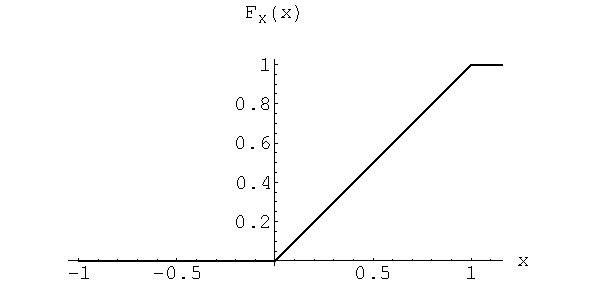
\includegraphics{distribucionuniforme}
\end{center}
\caption{Función de distribución de una v.a. uniforme en el intervalo unidad.}
\end{figure}

Por ejemplo $$F_{x}(0.75)=0.75$$
\end{example}



En las variables continuas los sucesos del tipo $\{X\leq x \}$ y $\{X< x \}$ tendrán la
misma probabilidad, y otros tipos de sucesos similares también, algunas de estas
propiedades se explicitan en la siguiente proposición.

\begin{proposition}
    Dada una v.a. continua $X$ se tiene que:
\begin{enumerate}[a)]
    \item $P(X\leq b)=P(X<b)$
    \item $P(X<b)=P(X<a)+P(a<X<b)$
    \item $P(a<X<b)=P(X<b)-P(X<a)$
\end{enumerate}
\end{proposition}

\textbf{Demostración:}
\begin{itemize}
    \item[b)] $\{X<a\}\cap \{a<X<b\}=\emptyset$
$\{X<a\}\cup \{a<X<b\}=\{X<a\}$ entonces\newline
$$P(X\leq b)=P(\{X<a\}\cup \{a<X<b\})=P(X<a)+P(a<X<b)$$
    \item[a)] $P(X<b)=P(X<b)+P(X=b)=P(X<b)$
    \item[c)] \'Idem que b) aplicando a).
\end{itemize}

Las propiedades anteriores  y combinaciones de ellas se pueden
escribir utilizando la función de distribución de $X$:

\begin{proposition}Dada una variable aleatoria continua se tiene que:
    \begin{enumerate}[a)]
        \item $F_{X}(b)=F_{X}(a)+P(a<X<b)$
        \item $P(a<X<b)=F_{X}(b)-F_{X}(a)$
         \item $P(a\leq X\leq b)=F_{X}(b)-F_{X}(a)$
     \end{enumerate}
     \end{proposition}

    \textbf{Demostración:} ejercicio.

\begin{example}
    En los dardos:
    $$P(0.25<X<0.3)=F_{X}(0.3)-F_{X}(0.25)=$$
    $$=0.3-0.25=0.05$$
\end{example}

\subsection{Función de densidad}

Una función $f:\RR\to\RR$ es una función de densidad sobre $\RR$ si cumple que

\begin{enumerate}[a)]
\item $f_{X}(x)\geq 0$ para todo $x \in\RR.$
\item $f$ es continua salvo a lo más en una cantidad finita de puntos sobre
 cada intervalo acotado de $\R$, es decir es
integrable Riemman.
\item $\int\limits_{-\infty}^{+\infty} f_{X}(x) dx=1.$
\end{enumerate}

\begin{definition}

Sea $X$ una v.a. con función de distribución $F_X$. Sea $f:\RR\to\\R$ una función de
densidad tal que
$$F_X(x)=\int_{-\infty}^{x} f_X(t) dt.\mbox{ para todo } x\in\RR.$$

Entonces $X$ es una variable aleatoria continua y $f_X$ es la densidad de la v.a.  $X$.

El conjunto $D_X=\{x\in\RR| f_x(x)>0\}$ recibe el nombre de soporte o dominio de la
variable aleatoria continua y se interpreta su conjunto de resultados posibles.
\end{definition}

 \begin{example}
    En nuestra diana la función $f$ es una densidad
    $$f_{X}(x)=\left\{
    \begin{array}{ll}
        0 & \mbox{si } x\leq 0\\
        1 & \mbox{si } 0 < x < 1\\
        0 & \mbox{si } 1\leq x
     \end{array}\right.
    $$

     que    es la densidad de $X$, en efecto:

\begin{itemize}
\item Si $x \leq 0$ entonces $\int_{-\infty}^x f_X(t) dt = 0.$
\item  Si $0\leq x\leq 1$ entonces $\int_{-\infty}^x f_X(t) dt =
\int_{0}^x 1 dt = x.$
\item Si $x\geq 1$  entonces $\int_{-\infty}^x f_X(t) dt =
\int_{0}^1 1 dt = 1.$
\end{itemize}


Luego $F_X(x)=\int_{-\infty}^x f_X(t) dt$ para todo $x\in\RR.$

\end{example}

        \begin{figure}
       \begin{center} 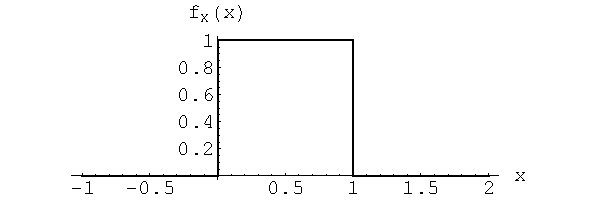
\includegraphics{densidaduniforme}
\end{center}
        \caption{Función de densidad de una v.a. uniforme en el intervalo
    $(0,1)$}
\end{figure}


La función de densidad nos permite calcular diversas probabilidades.

\begin{proposition} Sea $X$ una v.a. continua con función de distribución $F_X$ y de
densidad $f_X$, entonces
\begin{enumerate}
 \item $P(a< X< b)=P(a<X\leq b)= P(a\leq X< b)= P(a\leq X\leq b)=\int_{a}^b f_X(x) dx.$
\item Si $A$ es un recinto adecuado\footnote{ Un boreliano} de $\RR$ entonces $P(X\in
A)=\int_{A} f(x) dx=\int_{A\cap D_X} f(x) dx$.
\end{enumerate}
\end{proposition}


La siguiente proposición fija algunas propiedades de la función de densidad para v.a.
continuas y nos da un método de cálculo; la densidad es la derivada de la función de
distribución.

\begin{proposition}

Sea $X$ una v.a. continua con función de distribución $F_X$ y de densidad $f_X$, entonces:

\begin{enumerate}[a)]
\item $F_X$ es continua.
\item Si $f_x$ es continua en un punto $x$, $F_X$ es derivable en ese punto y
$F_X'(x)=f_X(x).$
\item $P(X=x)=0$ para todo $x\in\RR.$
\end{enumerate}
\end{proposition}
      %%%  \textbf{Ejercicio:} Comprobar estas propiedades en la diana.

        \begin{example}
            Sea $X=$ tiempo de ejecución de un proceso. Se supone que $X$
             sigue una distribución uniforme en dos unidades de tiempo,
             si tarda más el proceso se cancela. Entonces

        $$F_{X}(x)=P(X\leq x)=\frac{CF}{CP}=\frac{x}{2}$$
        Luego su función de distribución es:



            $$F_{X}(x)=\left\{\begin{array}{ll}
        0 & \mbox{si } x\leq 0\\
        \frac{x}{2} & \mbox{si } 0<x<2\\
        1 & \mbox{si } 2\leq x
        \end{array}\right.$$

        mientras que su función de densidad es:
            $$f_{X}(x)=F_{X}'(x)=\left\{\begin{array}{ll}
        0 & \mbox{si } x\leq 0\\
        \frac{1}{2} & \mbox{si } 0<x\leq 2\\
        0 & \mbox{si } 2\leq x
        \end{array}\right.$$

                Efectivamente
\begin{itemize}
                \item $f_{X}(x)\geq 0,$ y tiene un conjunto finito de discontinuidades.
                \item $F_X(x)=\int_{-\infty}^x f_X(t) dt.$ para todo $x\in \RR$ (ejercicio,
                resolverlo gráficamente.)
                \item $\int\limits_{-\infty}^{+\infty}f_{X}(x)dx=
                \int\limits_{0}^{2}\frac{1}{2}dx=\frac{x}{2}\mid_{0}^{2}=
                =\frac{2}{2}-\frac{0}{2}=1.$
\end{itemize}
\end{example}

        \textbf{Ejercicio:} Calcular la probabilidad de que uno de nuestros procesos tarde
        más de una unidad de tiempo en ser procesado. Calcular también la  probabilidad de
         que dure entre $0.5$ y $1.5$ unidades de tiempo.

         \section{Momentos para variables aleatorias continuas}
Los mismos comentarios y definiciones que se dieron en la sección correspondiente del tema
de estadística descriptiva %\ref{modis}
 son aplicables aquí. Así que sólo daremos las
definiciones, la forma de cálculo y algunos ejemplos.


    \subsection{Esperanza de  una v.a. continua}
    Sea $X$ una v.a. continua con función de densidad $f_{X}(x)$
    entonces:

    \begin{itemize}
    \item su esperanza es :
    $E(X)=\int\limits_{-\infty}^{+\infty} xf_{X}(x)dx.$
    \item Si $g(x)$ es una función de la variable $X$ entonces
    $$E(g(X))=\int\limits_{-\infty}^{+\infty} g(x)f_{X}(x)dx.$$
    \end{itemize}

    \subsection{Varianza  de una  v.a. continuas}
        \begin{itemize}
            \item $Var(X)=\sigma_{X}^{2}=E((X-\mu_{X})^2)=
            \int\limits_{-\infty}^{+\infty} (x-\mu_{X})^2 f_{X}(x)dx.$
            \item A $\sigma_{X}=+\sqrt{\sigma_{X}^{2}}$ se le denomina desviación típica o
            estándar de $X$.
        \end{itemize}




\textbf{Propiedades}
\begin{itemize}
    \item $\sigma_{X}^{2}\geq 0$
    \item $Var(cte)=E(cte^2)-(E(cte))^2= cte^2 - cte^2=0$
    \item $Var(x)=E(X^{2})-\mu_{X}^2=\int\limits_{-\infty}^{+\infty}x^2
    f_{X}(x)dx - \mu_{X}^2.$
    \item El mínimo de $E((X-C)^2)$ se alcanza cuando $C=E(X)$ y es $Var(X)$.
    \end{itemize}

    \textbf{Ejemplos} Calcular $\mu_{X}$ y $\sigma_{X}^{2}$ en el dardo.

    Resultado $\mu_{X}=\frac{1}{2}$, $E(X^2)=\frac{1}{3}$,
    $Var(X)=\frac{1}{12}$.

%\section{Transformación de variables aleatorias}
    \subsubsection{Esperanza y varianza de trasformaciones lineales}
    Sea $X$ una v.a. continua con $E(X)=\mu_{X}$ y $Var(X)=\sigma_{X}^{2}$ sea $Y=a+b X$, donde
$a,b\in\RR$, es una nueva v.a. continua obtenida mediante una transformación lineal de $X$.
Se verifican las mismas propiedades que en el caso discreto:
 \begin{itemize}
     \item  $E(Y)=E(a+b X)=a+b E(X)$
     \item $Var(Y)=Var(a+b X)=b^{2} Var(X)$
      \item $\sigma_{Y}=|b| \sigma_{X}$
      \item $Z=\frac{X-\mu_{X}}{\sigma_{X}}$ es una transformación
      lineal de $X$ de forma que
      $$E(Z)=0 \mbox{ y } Var(Z)=1$$
 \end{itemize}

            \textbf{Ejemplo}
            En una empresa de venta de vinos por internet, sea
            $X=$ número de  litros de vino del país vendidos en un año.
            Supongamos que sabemos que $E(X)=10000$ y que $Var(X)=100$
            Supongamos que los gastos fijos de distribución son
            50000 y el beneficio por litro es de 10 pts por botella.
            Definimos $T=10 X-50000$ que será el beneficio después de gastos
            entonces:
            $$E(T)=10 E(X)-50000 = 50000$$
            y
            $$Var(T)=10^2 VAR(X)= 10000$$


\section{Transformación de variables aleatorias}


          Muchas variables aleatorias son funciones de otras v.a. En lo que
          sigue resumiremos diversas técnicas para dada una v.a. $X$ y una
          transformación $Y=h(X)$  encontrar $F_{Y}$ a
          partir de $F_{X}$.


          \subsection{Transformaciones de v.a. discretas}

        \begin{proposition}
        Sea $X$ una v.a. discreta con \newline
        $X(\Omega)=\{x_{1},x_{2},\ldots,x_{n},..\}$ y sea $h:\R\to\R$ una aplicación.
        Entonces $Y=h(X)$ es también una v.a. discreta. Además si $P_X$
        y $F_{X}$ son las funciones de probabilidad y de distribución de
        $X$ entonces

        \begin{enumerate}[a)]
        \item $\displaystyle P_{Y}(y)=\sum_{x_{i}|h(x_{i})=y}P_X(x_{i}).$
        \item $\displaystyle F_{Y}(y)=\sum_{x_{i}|h(x_{i})\leq y} P_X(x_{i}).$
        \end{enumerate}
\end{proposition}

        \subsection{Transformaciones de v.a. continuas}

        Desafortunadamente este caso no es tan sencillo como el anterior, pues la
        transformación de una v.a. continua puede ser continua, discreta, mixta \ldots

        \begin{proposition}
        Sea $X$ una v.a. continua cuya función de densidad es $f_{X}$. Sea
        $h:\R\to\R$ una aplicación estrictamente monótona y derivable, tal
        que $h'(x)\not=0$ para todo $x\in\R$. Sea $Y=h(X)$ la
        transformación de $X$ por $h$. Entonces $Y$ es una v.a. continua con función
        de densidad

       $$f_{Y}(y)=\left.\frac{f_{X}(x)}
        {\left|h'(x)\right|}\right|_{x=h^{-1}(y)}$$
        \end{proposition}

   \begin{proposition}
    Sea $X$ una v.a. continua cuya función de densidad es $f_{X}$. Si
        $h:\R\to\R$ es  una aplicación, no necesariamente monótona,
         pero sí derivable con derivada no nula, y si
        la ecuación $h(x)=y$ tiene un número finito de soluciones
        $x_{1},x_{2},..,x_{n}$ entonces:

        $$\displaystyle f_{Y}(y)=\left.\sum_{k=1}^{n} \frac{f_{X}(x)}
        {\left|h'(x)\right|}\right|_{x=x_{k}}$$
     \end{proposition}

     \subsubsection{Método general}
        Cuando no podamos aplicar las propiedades anteriores intentaremos
        calcular primero la función de distribución de la transformación
        y luego su densidad.

        Notemos que en general si $Y=g(X)$ es una v.a. transformación  de la
        v.a. $X$ entonces

        $$F_{Y}(y)=P(Y\leq y)=P(g(X)\leq y)$$

        Por ejemplo si $g$ es estrictamente creciente y cont.

        $$F_{Y}(y)=P(g(X)\leq y)=P(X\leq g^{-1}(y))=F_{X}(g^{-1}(y))$$

        y si $g$ es estrictamente decreciente y cont.
        $$F_{Y}(y)=P(g(X)\leq y)=P(X\geq g^{-1}(y))=1-F_{X}(g^{-1}(y))$$



        \section{ Desigualdad de Chebyshef}

Veremos en esta sección distintas desigualdades que acotan determinadas probabilidades de
una variable aleatoria. Estas desigualdades sirven en algunos casos para acotar
probabilidades de determinados sucesos, también son interesantes desde el punto de vista
teórico y por ejemplo para justificar que la varianza es una mediada de la dispersión de
los datos
              \subsection{Desigualdad de Markov}
\begin{proposition}
              Sea $X$ una v.a. positiva con $E(X)$ finita. Entonces
              $P(X\geq a)\leq \frac{E(X)}{a}$ para todo $a>0$.
\end{proposition}
\textbf{Demostración: }

              Si $X$ es continua  y sólo toma valores positivos\newline
              $\displaystyle E(X)=\int_{-\infty}^{+\infty} x f_{X}(x)
              dx=\int_{0}^{+\infty} x f_{X}(x) dx=
              \displaystyle \int_{0}^{a} x f_{X}(x)
              dx+\int_{a}^{+\infty} x f_{X}(x) dx \geq \int_{a}^{+\infty} x
              f_{X}(x) dx \geq\displaystyle a \int_{a}^{+\infty}
              f_{X}(x) dx=a P(X\geq a)$

              de donde se sigue que  $P(X\geq a)\leq \frac{E(X)}{a}$

          \begin{corollary}
          Sea $X$ una v.a. con $E(X)$ finita entonces $P(|X|\geq a )\leq
          \frac{E(|X|)}{a}$. Para todo $a>0$
          \end{corollary}


          \subsubsection{Desigualdad de Chebyshef}
          \begin{proposition}
          Sea  $X$ una v.a.con $E(X)=\mu$ y $Var(X)=\sigma^2$ entonces

          $$P(|X-\mu|\geq a)\leq \frac{\sigma^{2}}{a^2}$$ para todo $a>0$
\end{proposition}
          \textit{Demostración}:

          Apliquemos la consecuencia de la desigualdad de Markov a la v.a.
          no negativa $Y^2=(X-\mu)^{2}$ entones

          $P(Y^2\geq a^2)\leq
          \frac{E(Y^2)}{a^2}=\frac{E((X-\mu)^{2})}{a^2}=
          \frac{Var(X)}{a^2}=\frac{\sigma^{2}}{a^{2}}$

          Por otra parte

          $$P(Y^2\geq a^2)=P(|Y|\geq a)= P(|X-\mu|\geq a)$$

           hecho que, junto con la desigualdad anterior,
          demuestra el resultado.



         \textbf{Observación:} Supongamos que $X$ es una v.a. con $Var(X)=0$
         entonces aplicando la desigualdad anterior

         $P(|X-E(X)|\geq a )=0$ para todo $a>0$ lo que implica que
         $P(X=E(X))=1$ luego la probabilidad de que $X$ sea
         constantemente $E(X)$ es 1. Lo que nos confirma la utilidad de la varianza es una
         medida de la dispersión de los datos.

         \begin{example}

         Se sabe que el tiempo de respuesta medio y la desviación típica de
         un sistema multiusuario  son 15 y 3 u.t.
         respectivamente. Entonces:

         $P(|X-15|\geq 5)\leq \frac{9}{25}=0.36$.

         Si substituimos $a$ por $a\sigma$ en la
         desigualdad de Chebyshef. Entonces nos queda:

         $P(|X-\mu|\geq a \sigma)\leq
         \frac{\sigma^2}{(a\sigma)^2}=\frac{1}{a^2}$

         Que es otra manera de expresar la desigualdad de Chebyshef.

         La desigualdad de Chebyshef también se puede escribir de al menos dos maneras más:

         $P(\mu-a\leq X\leq \mu+a)\geq 1-\frac{\sigma^2}{a^2}$

         $P(\mu-a\cdot \sigma\leq X\leq \mu+ a \cdot \sigma)$
\end{example}


\subsubsection{La varianza como medida de dispersión}
         Tomando la segunda expresión que hemos visto para la desigualdad de
         Chebyshef para distintos valores de $a>0$ tenemos la siguiente tabla.
\begin{center}
         \begin{tabular}{l|l}
             a & $P(|X-E(X)|\geq a \sigma)$\\
             \hline
             1 & $\leq 1$ \\
             2 & $\leq 0.25$ \\
             3 & $\leq 0.111$ \\
             4 & $\leq 0.0025$
             \end{tabular}
\end{center}
             Lo que se interpreta, por ejemplo para $a=2$,  como
             que dada una v.a. $X$ con cualquier distribución
             que tenga $E(X)$ y $Var(X)$ finitos
            la  pro\-ba\-bi\-li\-dad de que un valor se aleje de la media $\mu$ más de
             2 desviaciones típicas es menor o igual que $0.25$. Es decir
             sólo el 25\% de los valores estarán alejados de la media
             más de $2\sigma$  !sea cual sea la distribución de la v.a.!
